% Results section body.  Every number is a macro from numbers.tex, which is
% generated from results/*.csv -- see scripts/make_numbers.py.

From a \SI{3}{\degree} tilt on the nominal plant every controller balances
(\pidNomSettle--\lqrNomSettle\,\si{\second} median time to stay within
\SI{2}{\degree}): this usual regime does not discriminate.

\subsection{A \SI{2}{\milli\metre} asymmetry, and why it is fatal}

Give the plant a \SI{2}{\milli\metre} center-of-mass offset and the classical designs hold attitude perfectly
until they lose the cube (Fig.~\ref{fig:timeseries}). Both halves of
Proposition~\ref{prop:lean} are confirmed numerically. First, the disturbance is
small: the equilibrium lean is
$\theta^\star\simeq\sqrt{2/3}\,d/l=\leanTwoMm\,\si{\degree}$, and with momentum
management the measured steady tilt tracks it to \leanErr\,\si{\percent} over
$d\in[1,3]\,\si{\milli\metre}$ and the wheels stop charging. They stop at a
standing index that a proportional law necessarily leaves and that grows
linearly with $d$: $\etaSlopeFbl$, $\etaSlopeSmc$, $\etaSlopeBks$,
$\etaSlopePid$ and $\etaSlopeLqr$ per mm for FBL+LQR, SMC, backstepping, PID
and LQR (noise-free \SI{60}{\second} runs, nominal plant), within \etaPredErr\,\si{\percent}
(\etaPredErrNoise\,\si{\percent} with sensor noise)
of $Mgd/(\sqrt3\,k_hh_{\max})$ from \eqref{eq:mm} and \eqref{eq:lean} for the
four managed designs (FBL+LQR, SMC, backstepping, PID); FBL+LQR falls from \fblFirstFallMm\,\si{\milli\metre},
where that index exceeds \etaLim. Second,
the classical designs regulate $\btheta_e\!\to\!0$, which is not an equilibrium
of the disturbed plant, so they must supply $P\btau_d$ forever: their stored
momentum ramps linearly and \eqref{eq:tsat} predicts $t_{sat}\propto1/d$. We
measure $t_{sat}d=\tsatSlope\,\si{\second\milli\metre}$ against
\tsatPred\,\si{\second\milli\metre} from \eqref{eq:tsat}.

\begin{figure}[t]
\centering
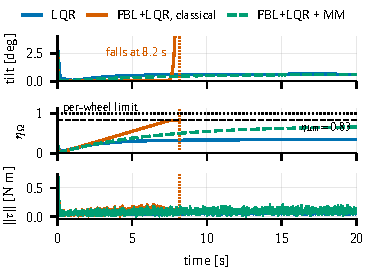
\includegraphics[width=0.72\columnwidth]{figures/fig_timeseries.pdf}
\caption{Corner balancing with a \SI{2}{\milli\metre} center-of-mass offset.
The classical FBL+LQR design (orange) tracks attitude until the
torque--speed envelope exhausts its accelerating authority, then falls; the same
design with momentum management (green, dashed) holds a small tilt that bleeds
the wheels through gravity. Middle: component-wise budget index
$\eta_\Omega=\max_i|\Omega_i|/\Omega_{\max}$: per-wheel limit dotted,
friction--envelope limit $\eta_{\lim}$ dashed. Tilt axis clipped at
\SI{4}{\degree}.}
\label{fig:timeseries}
\end{figure}

\subsection{Integral action on attitude does not rescue them}

A persistent disturbance is textbook integral territory, so a comparison in
which the nonlinear laws have no integrator would be rigged. Every design
therefore has an integral variant, tuned by the same protocol. It does not
help: over \mcSeeds{} perturbed plants the balanced-run
rate moves from \fblMcCl{} to \fblMcInt\,\si{\percent} for FBL+LQR,
\smcMcCl{} to \smcMcInt\,\si{\percent} for SMC and \backsteppingMcCl{} to
\backsteppingMcInt\,\si{\percent} for backstepping, and for the LQR it \emph{falls},
from \lqrMcCl{} to \lqrMcInt\,\si{\percent}. The PID already integrates.

The reason is exact: an unsaturated integrator on $\btheta_e$ makes
$\btheta_e=0$ the only candidate rest point, which
Proposition~\ref{prop:lean}(i) excludes when $P\btau_d\neq0$, so momentum ramps
at $P\btau_d$ whatever the gains. Integral action on stored momentum is a
different design, not tested here.

In these runs the classical designs never reach the wheel-speed limit. They fail at
$\eta_\Omega\approx\etaFall$, the terminal speed at which the accelerating
envelope \eqref{eq:envelope} only just covers bearing friction
($\eta_\Omega=\etaLim$, Sec.~\ref{sec:mm}); a model with only a hard speed
clamp would have predicted a longer survival. Fig.~\ref{fig:sweeps}
sweeps the asymmetry and the momentum budget. Sweeping $\Omega_{\max}$, the LQR balances down to
\lqrMinOmegaCl\,\si{\radian\per\second} while no classical nonlinear design
balances at \emph{any} budget in the swept range: their failure is not having
too little momentum but never releasing what they store. With the augmentation
they need \mmMinOmegaLo--\mmMinOmegaHi\,\si{\radian\per\second}.

\begin{figure}[t]
\centering
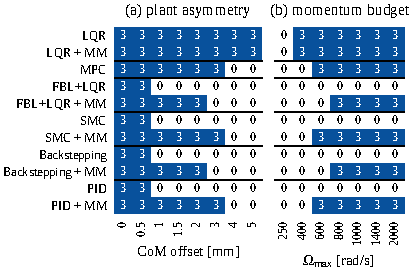
\includegraphics[width=0.80\columnwidth]{figures/fig_sweeps.pdf}
\caption{Runs that balance, out of 3 (sensor-noise seeds, \SI{3}{\degree}
initial tilt, \SI{20}{\second}), against (a)~the offset at
$\Omega_{\max}=\SI{1000}{\radian\per\second}$ and (b)~$\Omega_{\max}$ at
\SI{2}{\milli\metre} offset, without and with momentum management (MM).}
\label{fig:sweeps}
\end{figure}

\subsection{The signature of the invariant}

Fig.~\ref{fig:roa} maps recovery over initial tilt and pre-stored wheel momentum
(\SI{1}{\milli\metre} offset, \SI{25}{\second}),
separating momentum stored perpendicular to the balancing axis, which gravity
can dump, from momentum along the axis, which by Lemma~\ref{thm:invariant} it
cannot. Classical FBL+LQR, SMC, backstepping and PID recover \roaBlindCl\,\si{\percent} of the
sampled grid: at this offset they fall within the horizon from any initial state.

The invariant shows itself in how the augmented recovery depends on what is
already stored. With no stored momentum the two directions are
indistinguishable (\roaPerpZero{} against \roaVertZero\,\si{\percent}), as they must
be. Pooled over the five managed designs, as the pre-stored momentum grows the dumpable direction is unaffected
(\roaPerpHigh\,\si{\percent} beyond \SI{60}{\percent} of the budget) while recovery
along the invariant falls to \roaVertHigh\,\si{\percent}.

\begin{figure}[t]
\centering
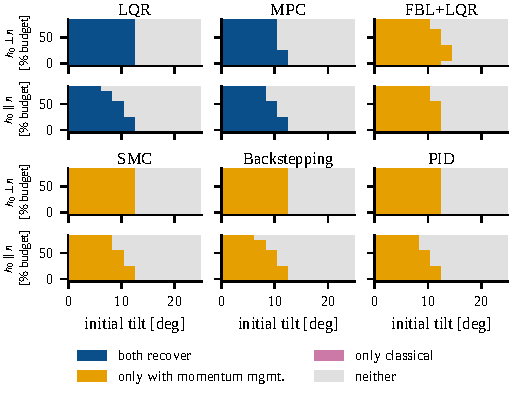
\includegraphics[width=0.75\columnwidth]{figures/fig_roa.pdf}
\caption{Empirical recovery map over initial tilt and pre-stored wheel
momentum $h_0$ (\SI{1}{\milli\metre} offset, \SI{25}{\second}, one seed per cell; not a
certified region of attraction):
momentum stored perpendicular to $\boldsymbol n$ (dumpable) above momentum
along $\boldsymbol n$ (the invariant of Lemma~\ref{thm:invariant}). Orange marks
states only the momentum-managed variant recovers: a band that does not shrink
with dumpable momentum and narrows as momentum along the invariant grows. MPC
has one variant (blue or grey). No cell is pink: on the sampled grid the augmentation never costs
a state the classical design already recovered.}
\label{fig:roa}
\end{figure}

\subsection{Perturbed plants, and a constrained benchmark}

Table~\ref{tab:main} reports \mcSeeds{} plants with
$\pm\SI{20}{\percent}$ on geometry, mass and dissipation parameters and a
center-of-mass offset
drawn per plant from $\mathcal{N}(1,1.5^2)$\,\si{\milli\metre} clipped at
$3\sigma$ (either sign). Episodes
last \mcHorizon\,\si{\second}, so survival is horizon-censored: every
momentum-blind survivor has $|d|\le\clSurvMaxOffset$\,\si{\milli\metre}, and managed
designs near their standing-momentum limit can also fall later. With the inertias recomputed from the drawn geometry, $h_{\max}$ varies by $-\SI{55}{\percent}/+\SI{40}{\percent}$ even though $\Omega_{\max}$ is fixed.

The three momentum-blind designs balance \backsteppingMcCl--\fblMcCl\,\si{\percent} of
plants. The LQR and the MPC weight stored momentum and the PID integrates, so none of
them is momentum-blind. With
momentum management, SMC reaches \smcMcMm\,\si{\percent}, PID
\pidMcMm\,\si{\percent}, backstepping \backsteppingMcMm\,\si{\percent} and
FBL+LQR \fblMcMm\,\si{\percent}. The MPC, with no
augmentation, reaches \mpcMcCl\,\si{\percent}. The LQR reaches
\lqrMcCl\,\si{\percent} on its own; adding the augmentation takes it to
\lqrMcMm\,\si{\percent}, a difference that is \emph{not} significant
(McNemar $p=1$); its tuned $k_h=\lqrKh$ makes the two variants nearly the same
controller. With the survival-first re-tuning of Sec.~\ref{sec:tuning} the
classical rates stay at \lexClLo--\lexClHi\,\si{\percent}, MPC at
\lexMpc\,\si{\percent}, the LQR moves to \lexLqrCl\,\si{\percent} (\lexLqrP),
and momentum management reaches \lexFblMm, \lexBksMm, \lexSmcMm{} and
\lexPidMm\,\si{\percent} for FBL+LQR, backstepping, SMC and PID (the first two
up from \fblMcMm{} and \backsteppingMcMm\,\si{\percent}, \lexFblP, McNemar; one optimizer run per design):
the gain comes from a larger $k_h$ (\num{0.16}$\to$\num{0.26} for FBL+LQR),
paid for in attitude error; exchanging $k_h$ alone reproduces it, so managed
survival is set mainly by $k_h$.
Table~\ref{tab:main} keeps the gains of the submitted study.

On paired plants (McNemar; hierarchical win ratio: survival, accuracy, time to
fall) momentum management wins \num{1.8}--\num{2.0} pairs per loss on FBL+LQR,
SMC, backstepping and PID ($p<10^{-3}$, Holm over fifteen tests). Where
both survive it is \emph{less} accurate (rank-biserial $r>0.85$): it pays for
survival with a permanent tilt.


\begin{table}[t]
\caption{Nominal and Monte-Carlo metrics, with Wilson \SI{95}{\percent}
intervals; Monte-Carlo rates depend on the offset distribution.
$^\dagger$median over runs that balanced.}
\label{tab:main}
\centering
\scriptsize
\setlength{\tabcolsep}{3.0pt}
\begin{tabular}{@{}llrrrcr@{}}
\toprule
& & \multicolumn{2}{c}{Nominal} & \multicolumn{3}{c}{Monte-Carlo} \\
\cmidrule(lr){3-4}\cmidrule(l){5-7}
Controller & Var. & $t_s$ [s] & $\int\|\tau\|^2$ & bal.\ [\%] & 95\,\% CI & IAE$^\dagger$ \\
\midrule
LQR & cl. & 0.08 & 0.010 & 99.3 & [96, 100] & 5.7 \\
LQR & MM & 0.08 & 0.010 & 100.0 & [97, 100] & 5.8 \\
MPC & cl. & 0.08 & 0.015 & 96.7 & [92, 99] & 5.2 \\
FBL+LQR & cl. & 0.06 & 0.102 & 36.0 & [28, 44] & 0.3 \\
FBL+LQR & MM & 0.06 & 0.105 & 82.0 & [75, 88] & 3.4 \\
SMC & cl. & 0.06 & 0.100 & 36.0 & [28, 44] & 0.4 \\
SMC & MM & 0.06 & 0.100 & 94.0 & [88, 97] & 4.7 \\
Backstepping & cl. & 0.06 & 0.131 & 34.7 & [27, 43] & 0.3 \\
Backstepping & MM & 0.06 & 0.131 & 85.3 & [78, 91] & 3.8 \\
PID & cl. & 0.06 & 0.243 & 33.3 & [26, 42] & 0.5 \\
PID & MM & 0.06 & 0.242 & 96.7 & [92, 99] & 5.1 \\
\bottomrule
\end{tabular}
\end{table}

\subsection{What the MPC baseline settles}

With the submitted gains the MPC outperforms managed FBL+LQR and backstepping
(22/0 and 17/0 discordant plants, McNemar $p<10^{-4}$) and ties managed SMC and
PID; after the re-tuning all are level. Momentum management buys no survival
advantage over the MPC. We make no computational claim.

The MPC never reaches its momentum bound (peak \num{858} of
\SI{1000}{\radian\per\second}): like the LQR, it is consistent with surviving through the lean its weight on
stored momentum induces; each of its five falls follows 16--18 solver
fallbacks. What
\eqref{eq:mm} adds is retrofit --- a reference offset leaving the inner loop
untouched --- which takes a PID from \pidMcCl{} to \pidMcMm\,\si{\percent}, level
with the MPC.

\subsection{Limitations}

Sweeping $b_p$ over three decades leaves the unloaded momentum identical to three
significant figures: the unloading is gravity, not pivot dissipation.
Four limitations bound the conclusions. The pivot is an ideal spherical joint
\ref{a:pivot}; a real vertex adds stiction, which widens the equilibrium of
Proposition~\ref{prop:lean} into $\theta^\star\pm\tau_s/(Mgl)$, adds a drilling
torque that breaks Lemma~\ref{thm:invariant}, and can slip.
The effect that does bite at this scale is a \emph{constant}
attitude-estimate bias $b$: since any equilibrium holds the true gravity-balance
attitude (Proposition~\ref{prop:lean}), \eqref{eq:mm} absorbs it as additional
standing momentum, to first order $Mgl\|Pb\|/k_h$, while a design regulating the
measured error to zero meets it as an offset. A bias of \SI{0.64}{\degree} is
torque-equivalent to the whole \SI{2}{\milli\metre} offset studied here, and
IMU-to-diagonal alignment on this class of machine is of that order. We model neither an estimator nor such a bias. No design can unload a
disturbance along $\bn$. The recoveries need pivot friction up to
$\mu\approx0.35$; $\eta_{\lim}$ depends on the unidentified bearing friction
(0.62 at $3b_w$); a \SI{1.1}{\percent} parallel-axis inertia omission changes
none of 120 paired outcomes. The nominal study is in-sample (a tuning scenario). And the study is entirely simulation-based.
